\section{Theorie}
\label{sec:Theorie}

Wird ein System aus seinem Ursprungszustand ausgelenkt, und kehrt es daraufhin, ohne zu oszillieren 
wieder in diesen zurück, so lässt sich dies als Relaxatationsvorgang beschreiben.
$A$ sei die Abweichung vom Ausgangszustand und $A(\infty)$ der Endzustand, der wieder dem Ausgangszustand
entspricht. Die zeitliche Änderung von $A$ ist dabei durch

\begin{equation}
    \label{eqn:dA}
    \frac{\text{d}A}{\text{d}t} = c\biggl[ A(t) - A(\infty) \biggr]
\end{equation}

zu beschreiben, woraus folgt: 
\begin{equation}
    \label{eqn:avont}
    A(t) = A(\infty) + \bigl[A(0) - A(\infty)]e^{ct}
\end{equation}

\FloatBarrier
\begin{figure}
    \centering
    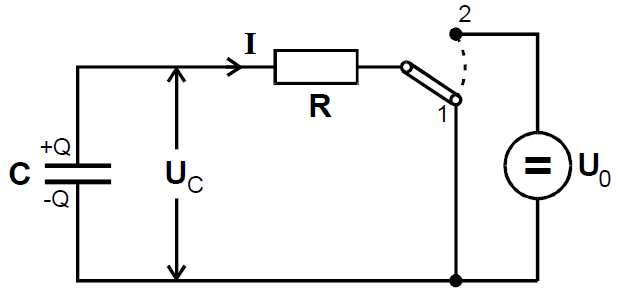
\includegraphics[height=6cm]{data/bild_1}
    \caption{RC-Kreis}
    \label{fig:bild_1}
\end{figure}
Anhand eines RC-Kreises wie in Abb \ref{fig:bild_1}, lassen sich Relaxatationsvorgänge durch das Auf- und Entladen des Kondensators
darstellen. Dabei gilt 
\begin{equation}
    U_C = \frac{Q}C   
\end{equation}
Durch die Spannung $U_C$ kommt ein Strom $I$ zustande, der über das ohm'sche Gesetz durch
\begin{equation}
    I = \frac{U_C}R 
\end{equation}
beschrieben wird. $I$ ist dabei auch die negative zeitliche Änderung der Ladung $Q$, wodurch man die folgende 
Differentialgleichung erhält.
\begin{equation}
    \frac{dQ}{dt} = -\frac{Q(t)}{RC}    
\end{equation}

Mit der Anfangsbedingung für den Entladevorgang
\begin{equation}
    Q(\infty) = 0
\end{equation}

gilt dann nach Gleichung \ref{eqn:avont} für den zeitlichen Verlauf der Ladung
\begin{equation}
    Q(t) = Q(0) e^{-t/{RC}}.
\end{equation}

Beim Aufladevorgang sind die Randbedingungen abweichend
\begin{align*}
    Q(0)        &= 0 \\
    Q(\infty)   &= CU_0 ,
\end{align*} wodurch $Q(t)$ in dem Fall durch
\begin{equation}
    Q(t) = CU_0 (1 - e^{-t/{RC}})
    \label{eqn:RC}
\end{equation}

beschrieben werden kann.

Die Zeitkonstante $RC$ gibt dabei die Geschwindigkeit an, mit der sich das System 
an den Endzustand $Q(\infty)$ annähert. Die Ladung $Q$ des Kondensators ändert sich während $\delta t=RC$ um
den Faktor
\begin{equation*}
    \frac{Q(t=RC)}{Q(0)} = \frac{1}e \approx 0,368 
\end{equation*} 


\begin{figure}
    \centering
    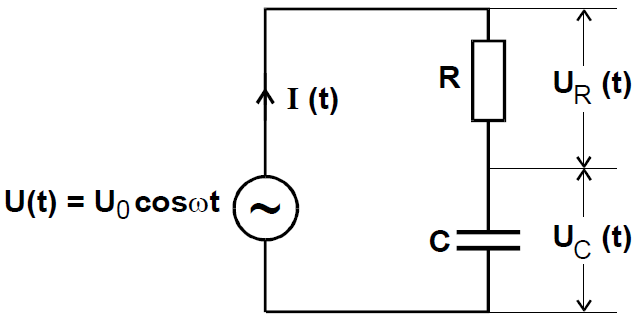
\includegraphics[height=6cm]{data/bild_2}
    \caption{RC-Kreis mit Wechselspannung}
    \label{fig:bild_2}
\end{figure}
\FloatBarrier
Relaxatationserscheinungen können auch in einem RC-Kreis, an dem eine Wechselspannung angeschlossen ist, betrachtet werden. 
Allgemein ist dabei \begin{equation}
    U(t) = U_0 \cos(\omega t)
\end{equation}, wobei $\omega$ die Kreisfrequenz ist. Wenn diese klein genug ist, bzw. wenn $\omega \ll 1/RC$, so ist $U_C (t)$
für alle $t$ näherungsweise gleich $U(t)$. Bei größeren Kreisfrequenzen kommt es durch den Widerstand $R$ zu einer Phasenverschiebung
$\phi$ zwischen der Kondensatorspannung und der Speisespannung. Die Zeit, die der Kondensator zum Auf- und Entladen hat, veringert sich 
außerdem mit steigendem $\omega$, wodurch die Spannungsamplitude des Kondensators $A$ abnimmt. Es gilt für die Kondensatorspannung 
\begin{equation}
    U_C (t) = A(\omega) \cos(\omega t + \phi(\omega))
\end{equation}

Damit lässt sich sowohl die Phasenverschiebung als auch die Amplitude der Kondensatorspannung in Abhängigkeit der Frequenz 
darstellen: \begin{equation}
    \phi = \arctan(-\omega RC)
    \label{eqn:phi}
\end{equation}
Für immer kleiner werdende Frequenzen geht $\phi$ dabei gegen null, und für $\omega \to \infty$ gegen $\pi/2$

\begin{equation}
    A(\omega) = \frac{U_0}{\sqrt{1 + \omega^2 R^2 C^2}}
    \label{eqn:A}
\end{equation}

Hierbei nähert sich, wie bereits erwähnt, $A$ für $\omega \to 0$ $U_0$ an, wobei es für $\omega \to \infty$ gegen null geht. 

Desweiteren ist ein RC-Kreis unter gewissen Umständen auch als Integrator für $U(t)$ zu gebrauchen. Ist $\omega \ll 1/RC$, so ist
$U_C \propto \int U(t)$. Über das zweite Kirchhoff'sche Gesetz lässt sich der Zusammenhang durch \begin{equation}
    U(t) = RC \frac{\text{d}U_C}{\text{d}t} + U_C (t)
\end{equation} darstellen.
Näherungsweise kann damit auch \begin{equation}
    U_C (t) = \frac{1}{RC} \int_0^t U(t') \text{d} t'
\end{equation} geschrieben werden.
